\documentclass{ecmorXV}
\usepackage{amsmath}
\usepackage{amsfonts}
\usepackage{mathrsfs}
%\usepackage{cite}
\usepackage{graphicx}
\usepackage{float}
\usepackage[font=footnotesize]{caption}
\usepackage{subfigure}
\usepackage{pifont}

\begin{document}

\section{Introduction}
\hspace{0.5cm}Often, most computational time in the simulation of multi-phase flow through porous media is taken up by
solution of the pressure equation. This involves primarily solving large systems of linear equations as 
part of the iterative solution of the time and space discretized governing nonlinear partial differential 
equations. The time spent in solving the linear systems depends on the size of the problem and the 
variations of permeability within the medium. Solution of problems with extreme contrast in the grid block 
permeability values may lead to very large computing times.\\
A potential approach to reduce the computing time for large-scale problems with the aid of Proper Orthogonal 
Decomposition (POD) is investigated in \cite{Astrid11} and \cite{Mark06}. Astrid et al. \cite{Astrid11} 
propose the use of a POD-based preconditioner for the acceleration  of the solution to the pressure equation. 
The preconditioner is constructed from a set of snapshots, obtained from solutions to the pressure equation 
in previous time steps. Once the snapshots are computed, the POD method is used to obtain a set of basis 
vectors that capture the most relevant features of the system, which can be used to improve the simulation 
time of the subsequent time steps. A similar approach is used in \cite{Mark06}, where a set of POD-based 
basis vectors is obtained from the initial time steps. However, in this case, the acceleration is 
achieved by only improving the initial guess.\\
Problems with a high contrast between the permeability coefficients are sometimes approached through the 
use of deflation techniques; see, e.g., \cite{Vuik99}. The use of deflation techniques involves the search 
of good deflation vectors, which are usually problem-dependent. In \cite{Vuik99}, subdomain based deflation 
vectors are used for layered problems with a large contrast between the permeability coefficients. However, 
these deflation vectors cannot be used if the distribution of the permeability coefficients  is not 
structured as is the case in, e.g., the well-known SPE 10 benchmark problem \cite{Christie01}.\\
Following the ideas of \cite{Astrid11} and \cite{Mark06}, we propose the use of POD of many snapshots to capture 
the system's behavior. The basis obtained with POD is studied as an alternative choice of deflation vectors 
to accelerate the convergence of the pressure solution in a porous medium with high-contrast variations in the 
permeability coefficients. As a first step, we consider incompressible single-phase flow through porous media 
with large variations in the permeability coefficients for layered academic problems and the SPE 10 benchmark.\\

\section{Method and/or Theory}
\subsection{Flow through porous media}
\hspace{0.5cm}We consider the semi-discretized form of the governing partial 
differential equations for single-phase flow, resulting in the system of 
ordinary differential equations \cite{Jansen13}, 
\begin{equation}\label{eq:trans}
 \mathbf{V}\dot{\mathbf{p}}+\mathbf{T}\mathbf{p}=\mathbf{q},
\end{equation}
where $\mathbf{p}$ is a vector of grid block potentials, $\mathbf{q}$ is a vector of grid block source terms (wells), 
the dot represents differentiation with respect to time, while $\mathbf{T}$ and 
$\mathbf{V}$ are the transmissibility and accumulation matrices.
If we neglect gravity, the potential reduces to pressure, and if we furthermore restrict the analysis to slightly 
compressible flow, the system of differential equations \eqref{eq:trans} is linear. 
In case of large compressibilities or multiphase-flow, the equations are nonlinear but can be solved iteratively 
using the Newton-Raphson (NR) method.\\
To solve Equation \eqref{eq:trans} it is necessary to define initial conditions and boundary conditions.
The latter conditions can be prescribed pressures (Dirichlet conditions), 
flow rates (Neumann conditions), or a combination of these (Robin conditions).\\
To represent the pressure drop resulting from sub-grid near-well flow convergence, and to allow for the 
prescription of pressures (rather than flow rates) in the wells we use the well-known 
Peaceman well model which changes Equation  \eqref{eq:trans} into
 \begin{equation}\label{eq:peac}
  \mathbf{V}\dot{\mathbf{p}} + \mathbf{T}\mathbf{p} = \mathbf{J}(\mathbf{p}-\mathbf{p}_{well}),
\end{equation}
where $\mathbf{J}$ is a matrix with well indices in the appropriate positions and $\mathbf{p}_{well}$ is a 
vector of well bore pressures \cite{Jansen13}. In case of incompressible flow, Equation \eqref{eq:peac} reduces to 
the system of algebraic equations 
 \begin{equation}\label{eq:peac1}
\mathbf{T}\mathbf{p} = \mathbf{J}(\mathbf{p}-\mathbf{p}_{well}).
\end{equation}
\subsection{Iterative solution methods}\label{syseq}
\hspace{0.5cm}Equation \eqref{eq:peac} can be numerically integrated, for which 
the implicit Euler formulation is the most popular time discretization method in the 
reservoir simulation community. This results in a time stepping sequence that 
requires the solution of a system of linear equations at each time step: 
\begin{equation}\label{eq:linsys}
 \mathbf{A}\mathbf{x}=\mathbf{b},
\end{equation}
where the vector $\mathbf{x} = \mathbf{p}_{k+1}$, and where $\mathbf{A}$ and $\mathbf{b}$ can be expressed in 
terms of $\mathbf{p}_k$, $\mathbf{T}$, $\mathbf{V}$, $\mathbf{J}$ and $\mathbf{p}_{well}$ \cite{Jansen13}. 
In case of a mass-conservative time discretization scheme for single-phase flow, $\mathbf{V}$ will be a 
function of $\mathbf{p}_{k+1}$, 
while in case of multi-phase flow also $\mathbf{T}$ and $\mathbf{J}$ become a function of $\mathbf{p}_{k+1}$. 
In those cases, system \eqref{eq:linsys} will be the result 
of a NR procedure, and multiple instances of it need to be solved during a single time step until the 
NR procedure has converged. In case of incompressible flow, the linear
system \eqref{eq:linsys} results directly from rewriting Equation \eqref{eq:peac1}. \\
System \eqref{eq:linsys} can be solved with direct or iterative methods.
Direct methods achieve a final solution, while the iterative ones
are stopped if the error is less than a given value. For realistically sized reservoir problems the use of iterative solvers is usually the most efficient 
and often the only possible choice. Some well-known iterative methods are: Jacobi, Gauss Seidel and, 
if the matrix is Symmetric Positive Definite (SPD), the Conjugate Gradient (CG) method.
Iterative methods can be preconditioned or deflated to accelerate the convergence. In the next section, 
we present the CG method, and we describe preconditioning and deflation techniques for the acceleration 
of this method.

\subsection*{Krylov subspace Methods}
\hspace{0.5cm}If we have two subspaces $\mathcal{K}_k,$ $\mathcal{L}_k$ of $\mathbb{R}^n$ and we want to solve 
 Equation \eqref{eq:linsys}, 
with $\mathbf{A} \in \mathbb{R}^{n\times n}$ we can use a projection method onto $\mathcal{K}_k$.
This method allows us to find an approximate solution $\mathbf{x}^k$ from an arbitrary initial guess 
 $\mathbf{x}^0$. This approximate solution lies in the Krylov subspace of dimension $k$ 
of the matrix $\mathbf{A}$ and residual $\mathbf{r}^0$,
\begin{equation*}
\mathbf{x}^k \in \mathbf{x}^0+\mathcal{K}_k(\mathbf{A},\mathbf{r}^0),
\end{equation*}
with $\mathcal{K}_k(\mathbf{A},\mathbf{r}^0)$ defined as:
\begin{equation*}
\mathcal{K}_k(\mathbf{A},\mathbf{r}^0)=span\{\mathbf{r}^0,\mathbf{A}\mathbf{r}^0,\dots,\mathbf{A}^{k-1}\mathbf{r}^0\},
\end{equation*}
where the residual $\mathbf{r}^k=\mathbf{b}-\mathbf{A}\mathbf{x}^k$ is orthogonal to the subspace $\mathcal{L}_k$, with 
\begin{equation*}
 \mathbf{x}^{k+1}=\mathbf{x}^k+\mathbf{B}^{-1}r^k, \qquad \mathbf{r}^k=\mathbf{b}-\mathbf{A}\mathbf{x}^k.
\end{equation*}
The subspace $\mathcal{L}_k$ is chosen depending on the Krylov subspace method that is used.


\subsection{Conjugate Gradient Method}
\hspace{0.5cm}The Conjugate Gradient (CG) method is a Krylov subspace method for $SPD$ matrices, such that
\begin{equation}\label{eq:CGm}
 ||\mathbf{x}-\mathbf{x}^k||_\mathbf{A} \footnote{$||\mathbf{x}||_\mathbf{A}= \sqrt{(\mathbf{x},\mathbf{x})_\mathbf{A}}=\sqrt{\mathbf{x}^T\mathbf{A}\mathbf{x}}.$} 
\end{equation}
is minimal, with $\mathbf{x}$ the solution of the system and $\mathbf{x}^k$ the approximate solution
after $k$ iterations. \\
\begin{table}[!ht]
\begin{tabular}{ |l| } 
\hline
  \textbf{Algorithm 1} Conjugate Gradient (CG) method, solving $\mathbf{A}\mathbf{x}=\mathbf{b}$.\\
  \hline
 \hline
\\
Give an initial guess $\mathbf{x}^0$. \\Compute $\mathbf{r}^0=\mathbf{b}-\mathbf{A}\mathbf{x}^0$ and set $\mathbf{p}^0=\mathbf{r}^0$.\\

\hspace{0.5cm}\textbf{for} $k=0,...,$ until convergence\\
 \hspace{1cm} $\alpha^k=\frac{(\mathbf{r}^{k},\mathbf{r}^{k})}{(\mathbf{A}\mathbf{p}^k,\mathbf{p}^k)}$\\
\hspace{1cm} $\mathbf{x}^{k+1}=\mathbf{x}^k+\alpha^k\mathbf{p}^k$\\
\hspace{1cm}$\mathbf{r}^{k+1}=\mathbf{r}^k-\alpha^k\mathbf{A}\mathbf{p}^k$\\
\hspace{1cm}$ \beta^k=\frac{(\mathbf{r}^{k+1},\mathbf{r}^{k+1})}{(\mathbf{r}^k,\mathbf{r}^k)}$\\
\hspace{1cm}$\mathbf{p}^{k+1}=\mathbf{r}^{k+1}+\beta^k\mathbf{p}^k$\\
\hspace{0.5cm}\textbf{end}\\
\hline
\end{tabular}
\end{table}
After $k+1$ iterations of the $CG$ method, the error of the iteration is bounded by:
\begin{equation}\label{eq:conv}
 ||\mathbf{x}-\mathbf{x}^{k+1}||_\mathbf{A}\leq 2||\mathbf{x}-\mathbf{x}^{0}||_\mathbf{A} 
 \left( \frac{\sqrt{\mathbf{C}_2(\mathbf{A})}-1}{\sqrt{\mathbf{C}_2(\mathbf{A})}+1} \right)^{k+1}.
 \footnote{The condition number $\mathbf{C}_2(\mathbf{A})$ is defined as  $\mathbf{C}_2(\mathbf{A})=
 \frac{\sqrt{\lambda_{max}(\mathbf{A}^T\mathbf{A})}}{\sqrt{\lambda_{min}(\mathbf{A}^T\mathbf{A})}}$. 
 If $\mathbf{A}$ is SPD, $\mathbf{C}_2(\mathbf{A})=\frac{\lambda_{max}(\mathbf{A})}{\lambda_{min}(\mathbf{A})}$.}
 \end{equation}
 \subsection{Preconditioning}
\hspace{0.5cm}If we want to accelerate the convergence of an iterative method, we can transform the system into
another one containing a better spectrum, i.e, a smaller condition number. 
This can be done by multiplying the original system \eqref{eq:linsys} by a matrix $\mathbf{M}^{-1}.$
\begin{equation}\label{eq:precon}
 \mathbf{M}^{-1}\mathbf{A}\mathbf{x}=\mathbf{M}^{-1}\mathbf{b}.
\end{equation}
The new system has the same solution but provides a substantial improvement on the spectrum. 
For this preconditioned system, the convergence is given by:
\begin{equation}\label{eq:convp}
 ||\mathbf{x}-\mathbf{x}^{k+1}||_\mathbf{A}\leq 2||\mathbf{x}-\mathbf{x}^{0}||_\mathbf{A} 
 \left( \frac{\sqrt{\mathbf{C}(\mathbf{M}^{-1}\mathbf{A})}-1}{\sqrt{\mathbf{C}(\mathbf{M}^{-1}\mathbf{A})}+1} \right)^{k+1}.
\end{equation}
$\mathbf{M}$ is an $SPD$ matrix chosen such that $\mathbf{C}(\mathbf{M}^{-1}\mathbf{A})\leq \mathbf{C}(\mathbf{A}),$ and $\mathbf{M}^{-1}b$ is easy to compute.

\subsection{Deflation}\label{def}
\hspace{0.5cm}Deflation is used to annihilate the effect of extreme eigenvalues on the convergence of an iterative method (\cite{Vuik99}). 
Given an $SPD$ matrix $\mathbf{A} \in \mathbb{R}^{n \times n}$, the deflation matrix $\mathbf{P}$ is defined as follows (\cite{Tang08}):
$$\mathbf{P}=\mathbf{I}-\mathbf{A}\mathbf{Q}, \qquad \mathbf{P} \in \mathbb{R}^{n \times n}, \qquad \mathbf{Q} \in \mathbb{R}^{n \times n},$$
where
$$\mathbf{Q}=\mathbf{Z}\mathbf{E}^{-1}\mathbf{Z}^T, \qquad \mathbf{Z} \in \mathbb{R}^{n \times m}, \qquad \mathbf{E} \in \mathbb{R}^{m \times m}, $$
with
$$\mathbf{E}=\mathbf{Z}^T\mathbf{A}\mathbf{Z}.$$
The matrix $\mathbf{E}$ is known as the $Galerkin$ or $coarse$ matrix that has to be invertible. 
If $\mathbf{A}$ is $SPD$ and $\mathbf{Z}$ is full rank then $\mathbf{E}$ is invertible. 
The full rank matrix $\mathbf{Z}$ is called the $deflation-subspace$ matrix, 
and it's $l<n$ columns are the
$deflation$ vectors or $projection$ vectors.\\
Some properties of the previous matrices are (\cite[pag. 27]{Tang08}):
\begin{enumerate}\label{defprop}
 \item[a)] $\mathbf{P}^2=\mathbf{P}.$
 \item[b)] $\mathbf{A}\mathbf{P}^T=\mathbf{P}\mathbf{A}.$
 \item[c)] $(\mathbf{I}-\mathbf{P}^T)\mathbf{x}=\mathbf{Q}\mathbf{b}.$
 \item[d)] $\mathbf{P}\mathbf{A}\mathbf{Z}=\mathbf{0}^{n\times m}.$
 \item[e)] $\mathbf{P}\mathbf{A}$ is $SPSD$\footnote{Symmetric Positive Semi-Definite, $(\mathbf{A}\mathbf{x},\mathbf{x})\geq 0$, for all $\mathbf{x}$.}.
\end{enumerate}
We can split the vector $\mathbf{x}$ as:
\begin{equation}\label{eq:splx}
    \mathbf{x}=\mathbf{I}\mathbf{x}-\mathbf{P}^T\mathbf{x}+\mathbf{P}^T\mathbf{x}=(\mathbf{I}-\mathbf{P}^T)\mathbf{x}+\mathbf{P}^T\mathbf{x}.
\end{equation}
Multiplying the expression above by $\mathbf{A}$, using the properties above, we have:
\begin{align*}
\mathbf{A}\mathbf{x}&=\mathbf{A}(\mathbf{I}-\mathbf{P}^T)\mathbf{b}+\mathbf{A}\mathbf{P}^T\mathbf{x},\qquad&Property:\\
\mathbf{A}\mathbf{x}&=\mathbf{A}\mathbf{Q}\mathbf{b}+\mathbf{A}\mathbf{P}^T\mathbf{x},&c)\\
\mathbf{b}&=\mathbf{A}\mathbf{Q}\mathbf{b}+\mathbf{P}\mathbf{A}\mathbf{x},&b),
\end{align*}
multiplying by $\mathbf{P}$ and using the properties $\mathbf{P}\mathbf{A}\mathbf{Q}=
\mathbf{0}^{n\times n}$ and $\mathbf{P}^2=\mathbf{P}$, properties $d$) and $e$), we have:
\begin{align}\label{eq:defsys}
\mathbf{P}\mathbf{A}\mathbf{Q}\mathbf{b}+\mathbf{P}^2\mathbf{A}\mathbf{x}&=\mathbf{P}\mathbf{b},\nonumber \\
\mathbf{P}\mathbf{A}\mathbf{x}&=\mathbf{P}\mathbf{b},
\end{align}
where $\mathbf{P}\mathbf{A}\mathbf{x}=\mathbf{P}\mathbf{b}$ is the deflated system. Since 
$\mathbf{P}\mathbf{A}$ is singular, the solution $\mathbf{x}$ can contain
components of the null space of $\mathbf{P}\mathbf{A}$. A solution to this system, called deflated
solution, is denoted by $\mathbf{\hat{x}}$.
The deflated system for $\mathbf{\hat{x}}$ is:
\begin{align}\label{eq:defsol}
\mathbf{P}\mathbf{A} \hat{\mathbf{x}}=\mathbf{P}\mathbf{b}.
\end{align}
As mentioned above, the solution to Equation \eqref{eq:defsys} can contain components of 
$\mathcal{N}(\mathbf{P}\mathbf{A})$. Therefore, a solution to Equation \eqref{eq:defsol},
$\mathbf{\hat{x}}$ can be decomposed as:
\begin{equation}\label{eq:xxy}
\mathbf{\hat{x}}=\mathbf{x}+ \mathbf{y},
\end{equation}
with $\mathbf{y} \in \mathcal{R}(\mathbf{Z})\subset \mathcal{N}(\mathbf{P}\mathbf{A}),$ 
and $\mathbf{x}$ the solution to Equation \eqref{eq:linsys}.\\
Note: If $\mathbf{y} \in \mathcal{R}(\mathbf{Z}),$ then $$\mathbf{y}=\sum^{m}_{i=1}\alpha_i \mathbf{z}_i,$$\\
 \begin{equation}\label{eq:paz}
 \mathbf{P}\mathbf{A}y=\mathbf{P}\mathbf{A}(\mathbf{z}_1\alpha_1 +...+ \mathbf{z}_m\alpha_m)=\mathbf{P}\mathbf{A}\mathbf{Z}\mathbf{\alpha},\end{equation}
 from \ref{defprop} h) $\mathbf{P}\mathbf{A}\mathbf{Z}=\mathbf{0}^{n\times l},$ then 
 \begin{equation}\label{eq:pay}
 \mathbf{P}\mathbf{A}\mathbf{y}=\mathbf{0}.
 \end{equation}
Therefore $\mathcal{R}(\mathbf{Z})\subset \mathcal{N}(\mathbf{P}\mathbf{A}).$ \\
Multiplying Equation \eqref{eq:xxy} by $\mathbf{P}^T$ we obtain:
$$\mathbf{P}^T\mathbf{\hat{x}}=\mathbf{P}^T\mathbf{x}+\mathbf{P}^T\mathbf{y},$$
combining Equation \eqref{eq:pay} with \ref{defprop} f), we have:
 \begin{equation*}
 \mathbf{P}\mathbf{A}y=\mathbf{A}\mathbf{P}^T\mathbf{y}=\mathbf{0}.
 \end{equation*}
 Therefore
  \begin{equation}\label{eq:ptx}
\mathbf{P}^T\mathbf{\hat{x}}=\mathbf{P}^T\mathbf{x}.
 \end{equation}
Substitution to Equation \eqref{eq:ptx} and \ref{defprop} g) in Equation \eqref{eq:splx} leads to:
\begin{equation}\label{eq:xfromxh}
    \mathbf{x}=\mathbf{Q}\mathbf{b}+\mathbf{P}^T\mathbf{\hat{x}}, 
\end{equation}
which gives us a relation between $\mathbf{\hat{x}}$ and $\mathbf{x}$.
 
\subsection{Deflated CG Method}
\hspace{0.5cm}To obtain the solution to the linear system \eqref{eq:linsys}, we solve the deflated system:
\begin{equation}\label{eq:deflsys}
    \mathbf{P}\mathbf{A}\hat{\mathbf{x}}=\mathbf{P}\mathbf{b}.
\end{equation}
with the CG method, for a deflated solution $\hat{\mathbf{x}}$. 
Therefore, the solution $\mathbf{x}$ to the original system is obtained from \eqref{eq:xfromxh}:
$$\mathbf{x}=\mathbf{Q}\mathbf{b}+\mathbf{P}^T\hat{\mathbf{x}}.$$
\subsection*{Deflated PCG Method}
The deflated linear system can also be preconditioned by an $SPD$ matrix $\mathbf{M}$.\\
The deflated preconditioned system to solve with CG is \cite[pag. 30]{Tang08}:
$$\tilde{\mathbf{P}} \tilde{\mathbf{A}} \hat{\tilde{\mathbf{x}}}=\tilde{\mathbf{P}}\tilde{\mathbf{b}},$$
where:
\begin{equation*}
 \tilde{\mathbf{A}}=\mathbf{M}^{-\frac{1}{2}}\mathbf{A}\mathbf{M}^{-\frac{1}{2}}, \qquad \hat{\tilde{\mathbf{x}}}=\mathbf{M}^{\frac{1}{2}}\hat{\mathbf{x}}, \qquad
 \tilde{\mathbf{b}}=\mathbf{M}^{-\frac{1}{2}}\mathbf{b}
\end{equation*}
This method is called the Deflated Preconditioned Conjugate Gradient $DPCG$ method, and the error is bounded by:
\begin{equation*}
 ||\mathbf{x}-\mathbf{x}^{i+1}||_\mathbf{A}\leq 2||\mathbf{x}-\mathbf{x}^{0}||_\mathbf{A} \left( \frac{\sqrt{\mathbf{C}_{eff}(\mathbf{M}^{-1}\mathbf{P}\mathbf{A})}-1}{\sqrt{\mathbf{C}_{eff}(\mathbf{M}^{-1}\mathbf{P}\mathbf{A})}+1} \right)^{i+1},
\end{equation*}
were $\mathbf{C}_{eff}=\frac{\lambda_{max}(M^{-1}PA)}{\lambda_{min}(M^{-1}PA)}$ is the effective condition 
number and $\lambda_{min}(M^{-1}PA)$ is the smallest non-zero eigenvalue of $M^{-1}PA$.
\subsection{Choices of Deflation Vectors}
\hspace{0.5cm}The deflation method is used to treat the most unfavorable eigenvalues
of $\mathbf{A}$. If the matrix $\mathbf{Z}$ contains eigenvectors corresponding to the unfavorable 
eigenvalues, the convergence of the 
iterative method is achieved faster. However, to obtain and to apply the eigenvectors is costly in most 
of the cases.
Therefore, a good choice of the matrix $\mathbf{Z}$ that does not contain the eigenvectors is essential
for the acceleration of the convergence.\\
A good choice of the deflation vectors is usually problem-dependent. Available information on the system is, in general,
used to obtain these vectors.
Most of the techniques used to choose deflation vectors are based on approximating eigenvectors, 
recycling (\cite{Clemens04}), subdomain deflation vectors (\cite{Vuik02}) or multigrid and 
multilevel based deflation techniques (\cite{Tang09,Smith96}). A summary of these techniques is given below.
\begin{description}
 \item [Recycling Deflation.] A set of vectors previously used is reused to build the deflation-subspace 
 matrix (\cite{Clemens04}). 
The vectors could be, for example, $q-1$
solution vectors of the linear system with different right-hand sides or of different time steps.
The matrix $\mathbf{Z}$ containing this solutions is:
$$\mathbf{Z}=[\mathbf{x}^{(1)},\mathbf{x}^{(2)},...,\mathbf{x}^{(q-1)}].$$
 \item [Subdomain Deflation.] The domain is divided into several subdomains,
 each corresponding to one or more deflation vectors.
For each subdomain, there is a deflation vector that has ones for points in the 
subdomain and zeros for points outside (\cite{Vuik02}).
 \item [Multi Grid and Multilevel Deflation.] For the multigrid and multilevel methods, 
 there are matrices called prolongation and restriction matrices that
allow us to pass from one level or grid to another. 
These matrices are used as the deflation-subspace matrices $\mathbf{Z}$ (\cite{Tang09}).
\end{description}

\subsection{Proper Orthogonal Decomposition (POD)}
\hspace{0.5cm}The Proper Orthogonal Decomposition (POD) 
method is a Model Order Reduction (MOR) method, where a high-order model is projected onto the space
spanned by a set of orthonormal basis vectors.
The high dimensional variable $\mathbf{x} \in \mathbb{R}^n$
is approximated by a linear combination of $l<<n$ orthonormal basis vectors \cite{Astrid11}:
\begin{equation}\label{eq4}
  \mathbf{x}\approx \sum_{i=1}^lz_i \mathbf{\phi}_i,
\end{equation}
where $\phi_i \in \mathbf{R}^n$ are the basis vectors and $z_i$ are their corresponding coefficients.
In matrix notation, equation \eqref{eq4} is rewritten as :
$$\mathbf{x}\approx \Phi\mathbf{z},$$
where $\Phi=[\phi_1 \text{ }\phi_2 \text{ }.. \text{ }\phi_l]$, $\Phi \in \mathbf{R}^{n\times l}$ 
is the matrix containing the basis vectors, and $\mathbf{z} \in \mathbf{R}^l$ is the vector 
containing the coefficients of the basis vectors. \\
The basis vectors are computed from a set of 'snapshots' $\{ \mathbf{x_i}\} _{i\in \mathbb{N}}$, 
obtained by simulation or experiments \cite{Mark06}. 
In POD, the basis vectors $\{ \mathbf{\phi} _j \} ^l _{j=1},$ are $l$ eigenvectors corresponding to 
the largest eigenvalues $\{ \mathbf{\lambda} _j \} ^l _{j=1}$ of the data snapshot correlation matrix $\mathbf{R}$.
\begin{equation}\label{eq:POD}
\mathbf{R}:= \frac{1}{m}\mathbf{X}\mathbf{X}^T \equiv \frac{1}{m} \sum_{i=1}^m \mathbf{x}_i \mathbf{x}_i^T,
\qquad \mathbf{X}:=[\mathbf{x}_1,\mathbf{x}_2,...\mathbf{x}_m],
\end{equation}
where $\mathbf{X}\in \mathbf{R}^{n\times m}$ is an SPSD matrix containing the previously obtained snapshots.
The $l$ eigenvectors should contain almost all the variability of the snapshots. 
Usually, they are chosen as the eigenvectors of the maximal number ($l$) of eigenvalues satisfying \cite{Mark06}:
\begin{equation}
\frac{\sum_{j=1}^l\lambda_j}{\sum_{j=1}^m\lambda_j}\leq \alpha, \qquad 0<\alpha \leq 1,
\end{equation}
with $\alpha$ close to 1. The eigenvalues are ordered from large to small with $\lambda_1$ 
the largest eigenvalue of $\mathbf{R}$.
\section{Results}
\subsection{Numerical experiments.}\label{numexp}
\hspace{0.5cm}These experiments are performed in order to understand the behavior of the Deflated Conjugate Gradient method 
preconditioned with Incomplete Cholesky (DICCG) and to find 
good deflation vectors for the given problems. We propose the use of snapshots and the snapshots-based 
basis functions of POD as deflation vectors.\\
In the present section, we give a general overview of the experiments that we perform, but the specifications
 are presented below for each problem separately. The reference solution is obtained with a direct solution method. 
 This solution is visually compared with the results obtained with the iterative solvers.\\
We observed that a good choice of snapshots, and therefore of deflation vectors, depends on the boundary 
conditions of the problem. Hence, we study two cases with different boundary conditions. 
For the first set of problems, Dirichlet boundary conditions are used for 
an academic layered model with various contrasts in permeability between the layers. 
In the second set of problems, we used Neumann boundary conditions (no-flux) for the previous academic
layered problem and for the SPE 10 benchmark problem. 
We investigate the behavior of the ICCG and DICCG methods with various contrasts between the 
permeability layers for both cases. \\
We study the influence of the size of the problem in the performance of the ICCG and DICCG methods 
changing the grid size of the second layer of the SPE 10 benchmark. 
We also investigate the performance of the above-mentioned methods 
with various tolerance values for the solvers. This study was performed for the second layer and 
for the complete SPE 10 benchmark (85 layers).
We also investigate the influence of the accuracy of the snapshots in 
the performance of the DICCG method for the complete SPE 10 benchmark.\\ \\
\emph{The model}\\
The experiments simulate flow through porous media with a constant porosity field of 0.2.
An incompressible single-phase model is
studied for a fluid with the following properties:
\begin{itemize}
 \item $\mu = 1 cp$
 \item $\rho = 1014 kg/m^3$
\end{itemize}
We model incompressible single-phase flow through porous media. The system of equations that describes 
this flow is given by Equation \eqref{eq:linsys}.\\
In these experiments, a Cartesian grid with different grid sizes is used. Wells or sources are added to the system. 
Neumann and Dirichlet boundary conditions are imposed. For some problems, a pressure drop is 
imposed in the $y$ direction (Dirichlet boundary condition), and for others, the no-flux (Neumann) boundary condition 
is used.
More specifications are presented below for each problem. 
The matrices corresponding to the linear systems $\mathbf{A}$ and right-hand sides $\mathbf{b}$ are obtained with MRST \cite{Lie13}.
\\ \\
\emph{Snapshots}\\
As mentioned above, for the DICCG method we need a set of deflation vectors. In a first series of
experiments, the deflation vectors are 
solutions of the system with various well configurations and boundary conditions. These solutions, 
called snapshots, are obtained with ICCG, the tolerance used is given for each problem. 
The configuration used to obtain each snapshot depends on the problem that we are solving. For each case,
the configuration of the snapshots, as well as the configuration of the system to solve, are presented.
\\ \\
\emph{The solver}\\
The solution of the system is approximated with ICCG and DICCG.\\
For the DICCG method, we need a set of deflation vectors. For the first case (Dirichlet and Neumann boundary conditions),
snapshots are used as deflation vectors. For the second case (Neumann boundary conditions only),
snapshots and basis vectors of POD are used as deflation vectors.
The tolerance or stopping criterium is taken as the 2-norm of the residual for the $k^{th}$ iteration divided by 
the 2-norm of the right-hand side of the preconditioned system: 
$$\frac{||\mathbf{M}^{-1}r^k||_2}{||\mathbf{M}^{-1}b||_2}\leq \epsilon.$$
The stopping criterium is varied for each problem. 
\\ \\
\emph{POD deflation vectors}\\
The POD method requires a basis for the projection of the high-order model. 
This basis contains the eigenvectors corresponding to the largest eigenvalues of the
data snapshot correlation matrix $\mathbf{R}$, as defined in Equation \eqref{eq:POD}.\\
In the second set of experiments (Neumann boundary conditions only), we use snapshots and the eigenvectors
corresponding to the two largest eigenvalues of the matrix $\mathbf{R}$ as deflation vectors.
The $\mathbf{x}_i's$ of the matrix $\mathbf{R}$ are the 
snapshots described in previous section. When we use POD deflation vectors for the DICCG method, 
we use the subscript $_{POD}$, i.e. the solver is DICCG$_{POD}$. 
\newpage
\textbf{\emph{Case 1, Dirichlet and Neumann boundary conditions.}}\\
In the configuration of \emph{Case 1}, four wells are positioned in a square at distances equal 
to one-third of the reservoir length and width. Two wells have a bottom hole pressure (bhp) of 5 bars, and two have 
a bhp of -5 bar. No-flux conditions are used at the right and left boundaries and a pressure drop
in the vertical direction. The pressure at the lower boundary ($y=1$) is 0 bars, and at
the upper boundary ($y=ny$) is 3 bars. 
The first four snapshots ($z_1-z_4$) are obtained setting only one well pressure
different from zero, taking no-flux conditions at the right and left boundaries and 
homogeneous Dirichlet conditions at the other boundaries. A fifth snapshot is obtained 
setting all the wells pressures to zero and setting a pressure drop in the vertical 
direction used for the
original system. 
A summary is presented below.
\begin{itemize}
\item[] Configuration 1:
\item[]  $System$ $configuration$ 
 \item[]  W1 =  W2 = -5 bars.
 \item[] W3 = W4 = +5 bars.
\item[] $Boundary$ $conditions:$
\item[] $P(y=1) = 0$ bars, $P(y=ny) = 3$ bars, $\frac{\partial P(x=1)}{\partial n}=\frac{\partial P(x=nx)}{\partial n}=0$.
\item[]  $Snapshots$ 
 \item[] $\mathbf{z}_1$: W1 = -5 bars, W2 = W3 = W4 = 0, 
\item[] $\mathbf{z}_2$: W2 = -5 bars, W1 = W3 = W4 = 0.
\item[] $\mathbf{z}_3$: W3 = +5 bars, W1 = W2 = W4 = 0.
\item[] $\mathbf{z}_4$: W4 = +5 bars, W1 = W2 = W3 = 0.
\item[] Boundary conditions for the first 4 snapshots: 
\item[] $P(y=1) =  P(y=ny) = 0$ bars, $\frac{\partial P(x=1)}{\partial n}=\frac{\partial P(x=nx)}{\partial n}=0$.
 \item[] $\mathbf{z}_5$: W1 =  W2 =  W3 = W4 = 0.
 \item[] Boundary conditions for the 5th snapshot: 
\item[] P(y=1) = 0 bars, P(y=ny) = 3 bars, $\frac{\partial P(x=1)}{\partial n}=\frac{\partial P(x=nx)}{\partial n}=0$.
\end{itemize}
\normalsize
\begin{figure}[!h]
\centering 
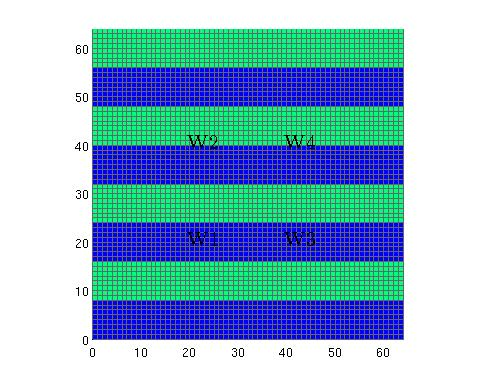
\includegraphics[width=5cm,height=5cm,keepaspectratio]
{perm_he_1.jpg}
\caption{ Heterogeneous permeability.}\label{fig:hep}
\end{figure}
\normalsize
As mentioned above, we studied flow through a porous medium with \emph{heterogeneous permeability} layers. A grid of
$nx = ny = 64$ elements is studied. We use 8 layers of the same size, 
4 layers with one value of permeability $\kappa_1$, followed by a layer with a different permeability value $\kappa_2$. 
The permeability of one set of layers is set to $\kappa_1=1mD$, the permeability of the other set $\kappa_2$ is changed. 
Therefore, the contrast in permeability between the layers $(\frac{\kappa_2}{\kappa_1}=\frac{\kappa_2}{1mD})$,
depends on the value of $\kappa_2$.\\
We investigate the dependence on the contrast in permeability value between the layers for the ICCG and DICCG methods.
The permeability of one set of layers is $\kappa_1=1mD$ in all cases, whereas the permeability of the other set of 
layers varies from $\kappa_2=10^{-1}mD$ to $\kappa_2=10^{-7}mD$. 
Figure \ref{fig:hep} shows these layers. The tolerance is set as $10^{-11}$ for the snapshots as well as for the original problem.\\ 
\normalsize
Table \ref{table:condn} shows the condition number for the matrix $A$, the preconditioned matrix $(M^{-1}A)$ and the deflated and preconditioned matrix 
$(M^{-1}PA)$ for various permeability contrasts between the layers.\\
\renewcommand{\arraystretch}{1.5}
\begin{table}[!ht]
\centering
\begin{tabular}{ |p{3cm}|p{1.5cm}|p{1.5cm}|p{1.5cm}|p{1.5cm}|  } 
 \hline
  $\kappa_2$ (mD) & $10^{-1}$& $10^{-3}$ & $10^{-5}$ & $10^{-7}$\\
  \hline
   $\mathbf{C}(A)$ & $2.6\times10^{3}$ & 2.4$\times10^{5}$&  $2.4\times10^{7}$&  $2.4\times10^{9}$\\ 
   \hline
 $\mathbf{C}(M^{-1}A)$  &$206.7$&$8.3\times10^{3}$&$8.3\times10^{5}$&$8.3\times10^{7}$\\
   \hline
  $\mathbf{C}_{eff}(M^{-1}PA)$ &$83.27$&$6\times10^{3}$&$1\times10^{6}$&$6\times10^{7}$\\
\hline
\end{tabular}
\caption{Table with the condition number for the matrix obtained solving the layered problem with 
various permeability contrasts between the layers. Original system,
preconditioned system and preconditioned and deflated system with five snapshots as deflation vectors (DICCG). 
Grid size of 32 x 32, $\kappa_1=1mD$.}
\label{table:condn}
\end{table}

Table \ref{table:he} shows the number of iterations required to achieve convergence 
for ICCG and DICCG, for various permeability contrasts between the layers.\footnote{The * means
that the solution is not achieved (from the plot of the solution). 
Meanwhile, ** means that the solution is close to the solution obtained with a direct solver.} \\
The solution is not reached when the value of permeability is greater than $\kappa_2=10^{-3}$ for both methods (ICCG and DICCG). 
For the ICCG method the solution is completely different from the solution obtained with a direct solver, 
whereas for the DICCG the solution is similar, but not the same. The plot of the residual and the solution 
to the problem are presented in Figures \ref{fig:convhe1} and \ref{fig:solhe1} for a value of permeability $\kappa_2=10^{-3}$.\\
As long as the correct solution is achieved ($\kappa_2=10^{-1},10^{-3}$), we note that the number of 
iterations increases when the contrast between the permeability layers increases for ICCG. For DICCG, 
we observe that we only need  one iteration despite the change in permeability contrast between the layers.\\
\begin{table}[!ht]
\centering
\begin{tabular}{ |p{1.5cm}|p{1.5cm}|p{1.5cm}|p{1.5cm}| p{1.5cm}|} 
\hline
 $\kappa_2$ (mD) & $10^{-1}$& $10^{-3}$ & $10^{-5}$ & $10^{-7}$\\
 \hline
  ICCG  & 75& 110&22*&22*\\ 
  DICCG  & 1 & 1& 10&4**\\ 
 \hline
\end{tabular}
\caption{Table with the number of iterations for different contrasts in the permeability of the layers
for the ICCG and DICCG methods.}
\label{table:he}
\end{table}
\begin{figure}[!h]
\centering
\begin{minipage}{.4\textwidth}
 \centering
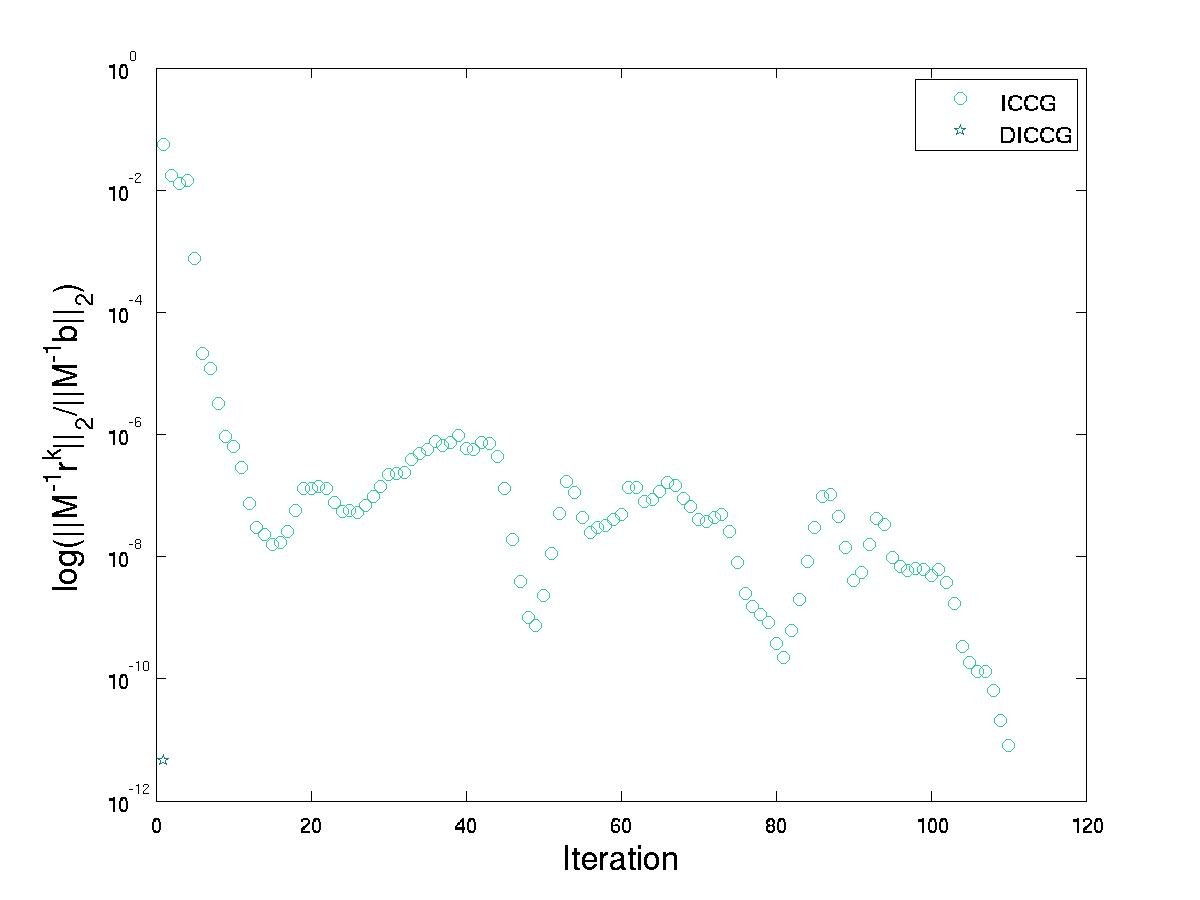
\includegraphics[width=6cm,height=6cm,keepaspectratio]
{conv_he_1.jpg}
\caption{Convergence for the heterogeneous problem, 64 x 64 grid cells,  $\kappa_2=10^{-3}mD$.}
\label{fig:convhe1}
\end{minipage}%
\hspace{1pt}
\begin{minipage}{.4\textwidth}
 \centering
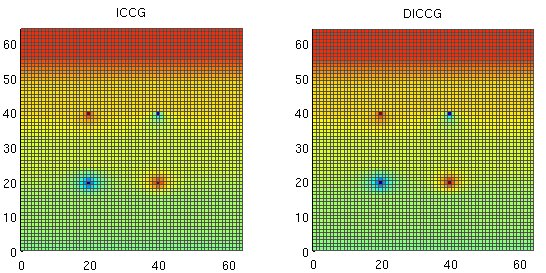
\includegraphics[width=6cm,height=6cm,keepaspectratio]
{sol_he_1.jpg}
\caption{Solution of the heterogeneous problem, 64 x 64 grid cells,$\kappa_2=10^{-3}mD$.}
\label{fig:solhe1}
\end{minipage}
\end{figure}

To better understand the cases when the solution has not been achieved, we study the error of the approximations.
If we want the relative error $e=\frac{||\mathbf{x}-\mathbf{x}^k||_2}{||\mathbf{x}||_2}$, with $\mathbf{x}$ the true
solution and $\mathbf{x}^k$ the approximation, to be less than $10^{-7}$, we need to choose a stopping criteria $(tol)$ 
so that $tol=e / \mathbf{C}_2(M^{-1}A)$ for the preconditioned system, and $tol=e  / \mathbf{C}_{eff}(M^{-1}PA)$ for the 
deflated and preconditoned system (see Appendix 1).\\ The tolerance is presented in Table \ref{table:tol} for the 
ICCG and DICCG methods. We observe that the required tolerance ($tol$) when $\kappa_2=10^{-5}mD, 10^{-7}mD$ is 
smaller than our choice ($tol= 10^{-11}$). As a consequence, we cannot expect to find a correct solution for these cases. 
\begin{table}[!ht]
\centering
\begin{tabular}{ |p{3cm}|p{1.5cm}|p{1.5cm}|p{1.5cm}|p{1.5cm}|  } 
 \hline
  $\kappa_2$ (mD) & $10^{-1}$& $10^{-3}$ & $10^{-5}$ & $10^{-7}$\\
  \hline
  $tol=\frac{e }{  \mathbf{C}(M^{-1}A)}$ &$5\times10^{-9}$&$1\times10^{-10}$&$1\times10^{-12}$&$1\times10^{-14}$\\
   \hline
 $tol=\frac{e}  { \mathbf{C}_{eff}(M^{-1}PA)}$ &$1\times10^{-8}$&$2\times10^{-10}$&$1\times10^{-12}$&$2\times10^{-14}$\\
\hline
\end{tabular}
\caption{Table with the tolerance for various permeability contrasts between the layers, grid size of 32 x 32, $\kappa_1=1mD$.}
\label{table:tol}
\end{table}

As we see from Table \ref{table:tol}, the tolerance required when $\kappa_2=10^{-5}mD$ is in the 
order of $10^{-12}$. Therefore, if we use this tolerance we can find the solution. 
Tolerance for the snapshots as well as for the solver is varied. We study 3 cases, in the first
case, the tolerance of the snapshots and the solvers is $10^{-12}$. In the second case, the 
tolerance of the snapshots is reduced to $10^{-14}$. Finally, in case 3 the tolerance of the 
solvers is reduced to $10^{-13}$. Table \ref{table:tol1} 
shows the number of iterations necessary to achieve convergence for ICCG and DICCG
for a given tolerance (Tol solver). The solution obtained with all the methods is visually 
compared with the solution obtained 
with a direct solver. \\
For ICCG, the solution obtained in the first two cases is similar to the expected solution but it 
is not the same which indicates that a tolerance of $10^{-13}$ is necessary to find the solution. 
For DICCG, in the first case, the solution is reached after eleven iterations. 
If we increase the accuracy of the 
snapshots (Case 2) we reach the correct solution for DICCG in one iteration (the dependence on the 
accuracy of the snapshots for the DICCG method is studied for the SPE 10 model in the next section). 
If we increase the accuracy of the solvers (Case 3), the solution is also achieved, but we note that 
for the deflation methods the number of iterations increases. 
\begin{table}[!ht]
\centering
\begin{tabular}{ |p{3cm}|p{1.5cm}|p{1.5cm}|p{1.5cm}| } 
\hline
Case &1&2&3\\ 
\hline
Tol snapshots &$1\times 10^{-12}$&$1\times10^{-14}$&$1\times10^{-14}$\\
   \hline
Tol solver &$1\times10^{-12}$&$1\times10^{-12}$&$1\times10^{-13}$\\

\hline
ICCG &$55^{**}$&$55^{**}$&$94$\\
   \hline
DICCG&$11$&$1$&$2$\\
\hline
\end{tabular}
\caption{Number of iterations for ICCG, DICCG for a layered problem, $\kappa_1=1mD$, $\kappa_2=10^{-5}mD$, grid size of 64x 64.}
\label{table:tol1}
\end{table}
\newpage
\textbf{\emph{Case 2, Neumann boundary conditions only.}}\\
In this case, four wells are positioned in the corners and have a bhp of -1 bar. One well
is positioned in the center of the domain and has a bhp of +4 bars
(see Figure \ref{fig:hep1}). We set Neumann boundary conditions in all boundaries. 
The snapshots ($z_1-z_4$) are obtained giving a value of zero to one well and non 
zero values to the other wells. 
A summary of the configurations is presented below.
\begin{itemize}
\item[] Configuration 2:
\item[]  $System$ $configuration$ 
 \item[]  W1 =  W2 = W3 = W4 = -1 bar.
 \item[] W5 = +4 bars.
\item[] $Boundary$ $conditions:$
\item[] $\frac{\partial P(y=1)}{\partial n}=\frac{\partial P(y=ny)}{\partial n}=\frac{\partial P(x=1)}{\partial n}=\frac{\partial P(x=nx)}{\partial n}=0$.
\item[] $Snapshots$
 \item[] $\mathbf{z}_1$: W1 = 0 bars, W2 = W3 = W4 =  -1 bars, W5 = +3 bars.
\item[] $\mathbf{z}_2$: W2 = 0 bars, W1 = W3 = W4 = -1 bars, W5 =  +3 bars.
\item[] $\mathbf{z}_3$: W3 = 0 bars, W1 = W2 = W4 = -1 bars, W5 =  +3 bars.
\item[] $\mathbf{z}_4$: W4 = 0 bars, W1 = W2 = W3 = -1 bars, W5 =  +3 bars.
 \item[] Boundary conditions 
\item[] $\frac{\partial P(y=1)}{\partial n}=\frac{\partial P(y=ny)}{\partial n}=\frac{\partial P(x=1)}{\partial n}=\frac{\partial P(x=nx)}{\partial n}=0$.
\end{itemize}
\normalsize

\emph{Heterogeneous permeability layers}\\
As in the previous case, single-phase flow through a porous medium with heterogeneous permeability layers is studied.
A grid of $nx = ny = 64$ elements is investigated. The deflation vectors used in this case are the 4 snapshots ($\mathbf{z}_1$-$\mathbf{z}_4$) and
two basis vectors obtained for the POD method.\\
The snapshots and the solutions are obtained with a tolerance of $10^{-11}$. \\\\
\begin{figure}[!h]
\centering
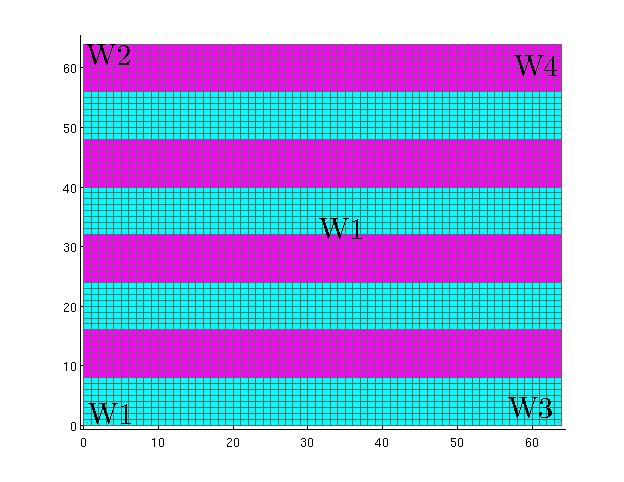
\includegraphics[width=5cm,height=5cm,keepaspectratio]
{perm_he_2.jpg}
\caption{ Heterogeneous permeability.}\label{fig:hep1}
\end{figure}

Table \ref{table:he2} shows the number of iterations required to achieve convergence 
for ICCG, DICCG with four snapshots as deflation vectors and DICC$G_{POD}$ with 2 POD basis vectors
as deflation vectors. The plot of the residual and the solution of the problem are presented in 
Figure \ref{fig:convhe2} and \ref{fig:solhe2} for the ICCG and DICCG methods.\\
As in Case 1, we note that the solution is not achieved when the permeability coefficient $\kappa_2$
is smaller than $10^{-3}$ for all the solvers. We can also observe that the performance of DICCG
and DICCG$_{POD}$ is similar. Therefore, in the analysis of the results, we will refer only to DICCG for
both solvers.
Studying solely the correct solutions for ICCG, the number of iterations 
increases as the contrast in the permeability increases. For the DICCG method, convergence is reached 
within one iteration.\\
\begin{table}[!ht]
\centering
\begin{tabular}{ |p{2.5cm}|p{1.5cm}|p{1.5cm}|p{1.5cm}| p{1.5cm}|} 
\hline
$\kappa_2$& $10^{-1}$ &$10^{-3}$  & $10^{-5}$ &$10^{-7}$\\
 \hline
  ICCG  & 90& 131&65*&64*\\ 
  DICCG  & 1 &1& 1*&1*\\ 
  DICCG$_{POD}$ & 1& 1& 1*& 1*\\
 \hline
\end{tabular}
\caption{Table with the number of iterations for different contrast in the permeability of the layers
for the ICCG, DICCG and DICCG$_{POD}$ methods, tolerance of solvers and snapshots $10^{-11}$. }
\label{table:he2}
\end{table}
\begin{figure}[!h]
\centering
\begin{minipage}{.4\textwidth}
 \centering
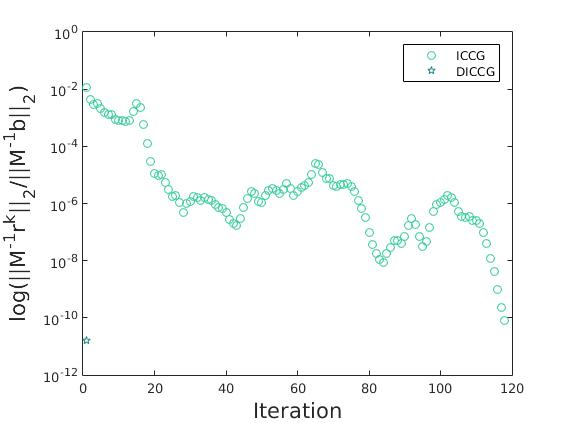
\includegraphics[width=5cm,height=5cm,keepaspectratio]
{conv_he_2.jpg}
\caption{Convergence for the heterogeneous problem, 64 x 64 grid cells, $\kappa_2=10^{-3}$.}
\label{fig:convhe2}
\end{minipage}%
\hspace{3 pt}
\begin{minipage}{.4\textwidth}
 \centering
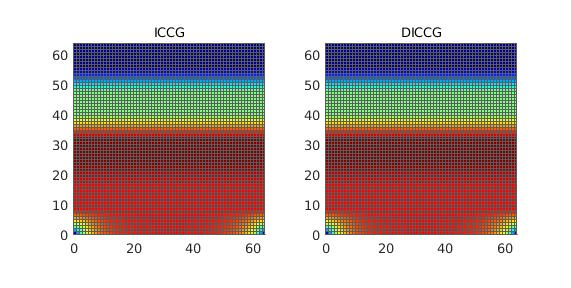
\includegraphics[width=6cm,height=6cm,keepaspectratio]
{sol_he_2.jpg}
\caption{Solution of the heterogeneous problem, 64 x 64 grid cells, $\kappa_2=10^{-3}$.}
\label{fig:solhe2}
\end{minipage}
\end{figure}

To better understand the utility of POD we present an example with a larger number of snapshots, and we use 
the POD basis vectors to reduce this number. We solve the heterogeneous layered case with layers of permeability 
$\kappa_1=1mD$ and $\kappa_2=(10^{-1}, 10^{-3})$ mD.
In this case, we use 15 snapshots that are not linearly independent.
These snapshots are the following:
\begin{itemize}
\item[] $Snapshots$ 
\item[] $\mathbf{z}_1$: W1 = W2 = W3 = W4 =  -1 bars, W5 =  +4 bars.
 \item[] $\mathbf{z}_2$: W1 = 0 bars, W2 = W3 = W4 =  -1 bars, W5 = +3 bars.
\item[] $\mathbf{z}_3$: W2 = 0 bars, W1 = W3 = W4 = -1 bars, W5 = +3 bars.
\item[] $\mathbf{z}_4$: W3 = 0 bars, W1 = W2 = W4 = -1 bars, W5 = +3 bars.
\item[] $\mathbf{z}_5$: W4 = 0 bars, W1 = W2 = W3 = -1 bars, W5 = +3 bars.
\item[] $\mathbf{z}_6$:  W1 = W2 = 0 bars,W3 = W4 = -1 bars, W5 =  +2 bars.
\item[] $\mathbf{z}_7$: W2 = W3 = 0 bars, W1 = W4 = -1 bars, W5 = +2 bars.
\item[] $\mathbf{z}_8$: W3 = W4 = 0 bars, W1 = W2 = -1 bars, W5 =  +2 bars.
 \item[] $\mathbf{z}_9$: W1 = W3 = 0 bars, W2 = W4 =  -1 bars, W5 = +2 bars.
\item[] $\mathbf{z}_{10}$: W2 = W4 = 0 bars, W1 = W3 = -1 bars, W5 =  +2 bars.
\item[] $\mathbf{z}_{11}$: W1 = W4 = 0 bars, W2 = W3 = -1 bars, W5 = +2 bars.
 \item[] $\mathbf{z}_{12}$: W1 = -1 bars, W2 = W3 = W4 =  0 bars, W5 =  +1 bars.
\item[] $\mathbf{z}_{13}$: W2 = -1 bars, W1 = W3 = W4 = 0 bars, W5 = +1 bars.
\item[] $\mathbf{z}_{14}$: W3 = -1 bars, W1 = W3 = W4 = 0 bars, W5 = +1 bars.
\item[] $\mathbf{z}_{15}$: W4 = -1 bars, W1 = W2 = W3 = 0 bars, W5 =  +1 bars.
 \item[] Boundary conditions 
\item[] $\frac{\partial P(y=1)}{\partial n}=\frac{\partial P(y=ny)}{\partial n}=\frac{\partial P(x=1)}{\partial n}=\frac{\partial P(x=nx)}{\partial n}=0$.
\end{itemize}

With these snapshots, we compute the data snapshot correlation matrix $\mathbf{R}=\mathbf{X}\mathbf{X}^T$,
where the rows of $\mathbf{X}$ are the snapshots presented above. We compute the eigenvalues of the correlation
matrix, they are presented in Figure \ref{fig:eig}. We observe that the first four eigenvalues 
are close to $10^8$ orders of magnitude larger than the rest of the eigenvalues. Our deflation vectors are 
the eigenvectors corresponding to these four eigenvalues.
\begin{figure}[!h]
 \centering
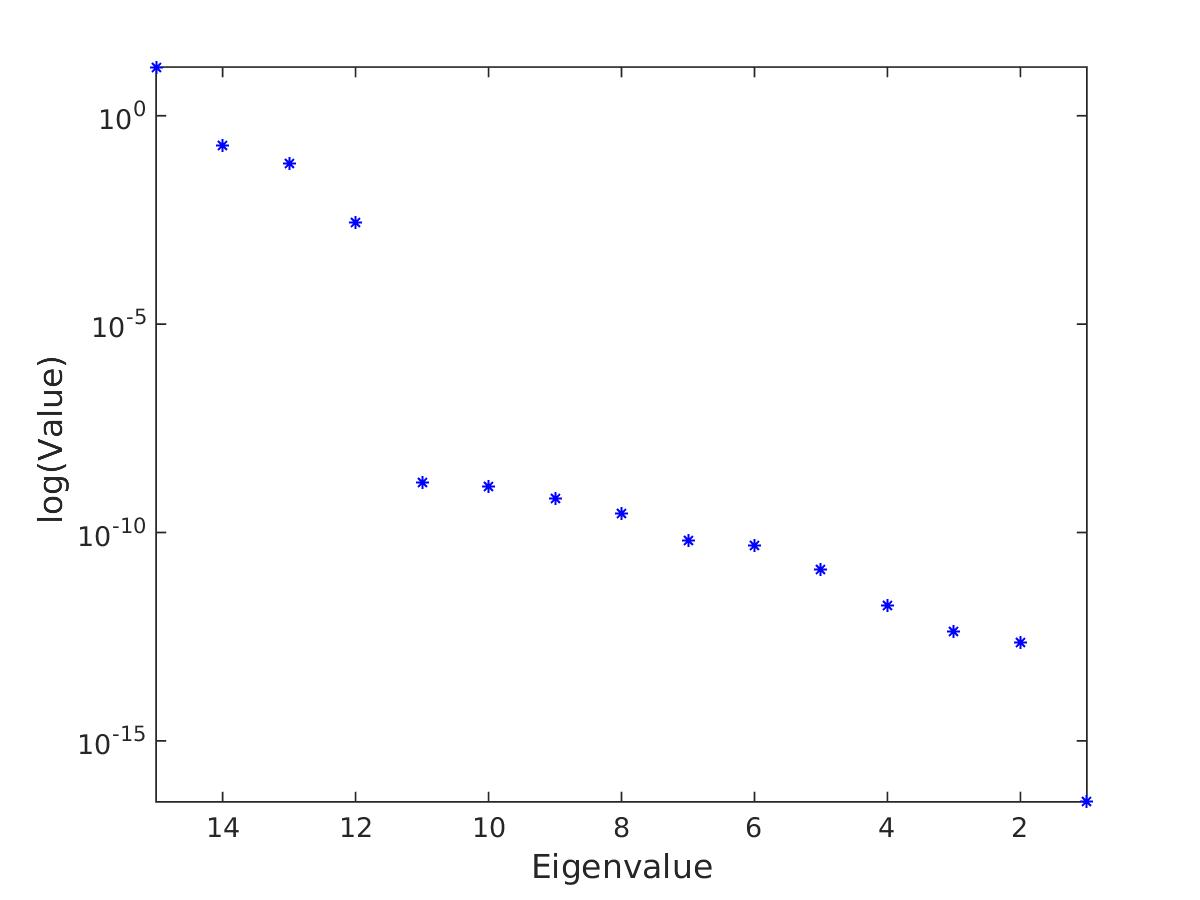
\includegraphics[width=6cm,height=6cm,keepaspectratio]
{eig_pod_het.jpg}
\caption{Eigenvalues of the snapshot correlation matrix $\mathbf{R}=\mathbf{X}\mathbf{X}^T$, 15 snapshots used.}
\label{fig:eig}
\end{figure}  
The number of iterations necessary to achieve convergence is presented in Table \ref{table:POD15} for the
ICCG and the deflated method. For the deflated method, 15 snapshots were used as deflation vectors DICCG$_{15}$,
and the eigenvectors corresponding to the 4 largest eigenvalues of the matrix $\mathbf{R}$ (see Figure \ref{fig:eig}). 
We observe that for the deflated method, when we use the 15 snapshots, the 
correct solution is not achieved after 500 iterations, the maximum number of iterations allowed for this problem.
For this problem we have a linearly dependent set of snapshots, causing that the
Galerkin matrix ($\mathbf{E}=\mathbf{Z}^T\mathbf{A}\mathbf{Z}$) is close to singular such that it cannot
be accurately inverted, a requirement for a good performance of the deflation method. 
As a result, the deflation method does not work properly.
However, when we use 4 of the basis vectors of POD, we achieve the 
solution within one iteration. In this example, we reduce the number of snapshots from 15 to 4 using 
the basis vectors of POD, selecting in this way the dominant features of the system.  
\begin{table}[!ht]
\centering
\begin{tabular}{ |p{2.5cm}|p{1.5cm}|p{1.5cm}|} 
\hline
$\kappa_2$& $10^{-1}$ &$10^{-3}$  \\
 \hline
  ICCG  & 90& 131\\ 
  DICCG$_{15}$  & 500* &500*\\ 
  DICCG$_{POD}$ & 1& 1\\
 \hline
\end{tabular}
\caption{Table with the number of iterations for different contrast in the permeability of the layers
for the ICCG, DICCG$_{15}$ and DICCG$_{POD}$ methods, tolerance of solvers and snapshots $10^{-11}$. }
\label{table:POD15}
\end{table}   
    
\newpage

\emph{SPE 10 model (1 layer)}\\
This model has large variations in the permeability coefficients.
It contains 60 x 220 x 85 cells, in this section only one layer (2nd) is used (60 x 220 x 1 cells).
This model has 5 sources or wells, four producers in the corners (negative) and one injector in the center (positive).
\\The snapshots are obtained solving the system with different well
configurations (\emph{Configuration 2}). Four snapshots are used as deflation vectors. As before,
we simulate single-phase incompressible flow.
The dependence of the DICCG method on the accuracy of the snapshots is investigated. Snapshots are obtained with different accuracy,
the values of tolerance used are
$10 ^{-1}$, $10 ^{-3}$, $10 ^{-5}$, and $10 ^{-7}$. The original system is solved with an accuracy of $10^{-7}$.
In the first experiment with the deflation method, the four snapshots are used as deflation vectors (DICCG). In the second, 
2 vectors of the POD basis are used as deflation vectors (DICCG$_{POD}$). 
\\ Different grid sizes are studied: 16 x 56, 30 x 110, 46 x 166 and 60 x 220.
\\Permeability is upscaled
averaging the permeability in each grid using the harmonic-arithmetic average algorithm from MRST.
The permeability of the coarser grid (16 x 56 cells) is shown in Figure \ref{fig:perm}.
The permeability contrast for the diverse grid size problems is shown in Table \ref{table:permgs}. 
From this table, we observe that the contrast in the permeability for different grid sizes varies slightly, but that the order
of magnitude remains the same for all the cases.\\
The condition number for the coarse grid problem (16 x 56) is studied in Table \ref{table:condnspe} for the 
original system, the preconditioned system and the deflated and preconditioned system with four snapshots as deflation vectors.
In this table we observe an important reduction in the condition number for the preconditioned the system
and a further reduction when the system is deflated.\\
\begin{figure}[!h]
\centering
\subfigure[16 x 56 grid cells]{
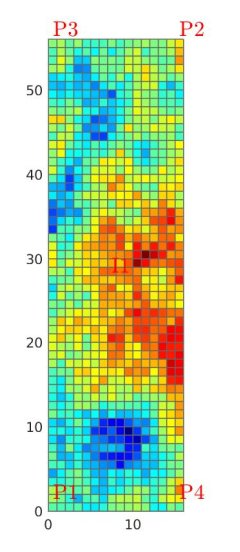
\includegraphics[width=6cm,height=6cm,keepaspectratio]
{perm_layer_2.jpg}
} \
\subfigure[60 x 220 grid cells]{
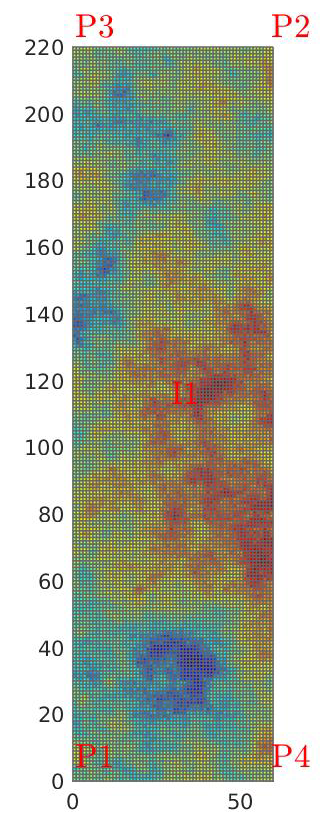
\includegraphics[width=6cm,height=6cm,keepaspectratio]
{perm_layer_22.jpg}
}
\caption{Permeability field, 16 x 56 and 60 x 220 grid cells.}\label{fig:perm}
\end{figure}

\begin{table}[!ht]
\centering
\begin{tabular}{ |p{2.5cm}|p{1.5cm}|p{1.5cm}|p{1.5cm}|p{1.5cm}|  } 
 \hline
  Grid size & 16 x 56 & 30 x 110 & 46 x 166 & 60 x 220\\
  \hline
  Contrast ($\times10^{7}$) & 1.04 & 2.52&  2.6&  2.8\\ 
\hline
\end{tabular}
\caption{Table with the contrast of permeabilities for
different grid sizes.}
\label{table:permgs}
\end{table}

\begin{table}[!ht]
\centering
\begin{tabular}{ |p{2.3cm}|p{2.3cm}|  } 
\hline
   Condition number &Value\\ 
   \hline
   $\mathbf{C}(A)$ &$2.2\times10^{6}$\\ 
   \hline
   $\mathbf{C}(M^{-1}A)$ &377\\ 
   \hline
 $\mathbf{C}_{eff}(M^{-1}PA)$  &82.7\\
\hline
\end{tabular}
\caption{Table with the condition number of the matrix obtained for the SPE 10 model. Original system,
preconditioned system and preconditioned and deflated system with four snapshots as deflation vectors (DICCG). 
Grid size of 16 x 56.}
\label{table:condnspe}
\end{table}
The number of iterations required to achieve convergence with the ICCG, DICCG and DICCG$_{POD}$ methods for various
grid sizes and various accuracy values of the snapshots is presented in Table \ref{table:itgrid}. \\
As in the previous experiment, the number of iterations is similar for the DICCG and DICCG$_{POD}$ methods,
therefore we will analyze only the solutions obtained with DICCG, as the same analysis holds for DICCG$_{POD}$.
\\The convergence and the solution to the ICCG and DICCG methods with a tolerance of the snapshots 
of $10^{-7}$ are presented in Figure \ref{fig:convspe} and Figure \ref{fig:solspe}. 
For ICCG, the required iterations to reach convergence increases as the size of the grid increases. 
We note that the accuracy of the snapshots is important for the DICCG method. 
When the accuracy is low, the DICCG method behaves almost as the ICCG method, 
as the accuracy increases, the number of iterations diminishes. We observe that, if we use the same 
accuracy for the snapshots and the solver, $10^{-7}$, the solution is reached within one iteration.  \\
\begin{table}[!ht]
\centering
\begin{tabular}{|p{1.5cm} |p{2cm}|p{1.5cm}|p{1.5cm}|p{1.5cm}|p{1.5cm}|  } 
 \hline
  Tol&Method  & 16 x 56 & 30 x 110 & 46 x 166 & 60 x 220\\
  \hline
  &ICCG                & 34 & 73&  126&  159\\ 
  \hline
$10 ^{-1}$ & DICCG & 33 & 72&  125 &  158 \\ 
 & DICCG$_{POD}$ & 33 & 72&  125 &  158 \\ 
  \hline
 $10 ^{-3}$ &DICCG& 18 & 38&  123&  151 \\ 
  & DICCG$_{POD}$ & 21 & 40&  123 &  153 \\ 
  \hline

$10 ^{-5}$ &  DICCG& 11 & 21&  27 &  55\\ 
 & DICCG$_{POD}$ & 11 & 21&  27 &  48 \\ 
   \hline

 $10 ^{-7}$  &DICCG & 1 & 1&  1 &  1 \\ 
  & DICCG$_{POD}$ & 1 & 1&  1 &  1 \\ 
\hline
\end{tabular}
\caption{Table with the number of iterations for ICCG, DICCG and DICCG$_{POD}$, various tolerance for the snapshots,
various grid sizes.}
\label{table:itgrid}
\end{table}
\begin{figure}[!h]
\centering
\begin{minipage}{.5\textwidth}
 \centering
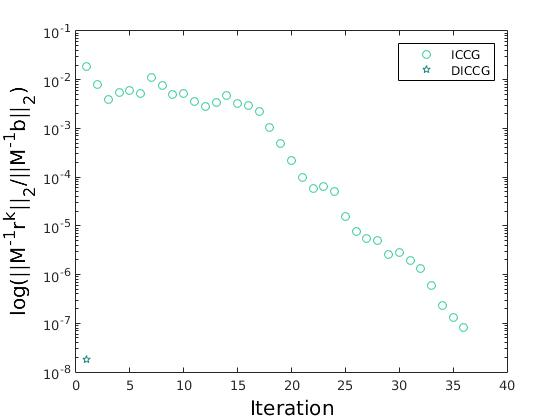
\includegraphics[width=6cm,height=6cm,keepaspectratio]
{conv_deftol-7_5_5.jpg}
\caption{Convergence for the SPE 10 problem, 16 x 56 grid cells, accuracy of the snapshots $10 ^{-7}$.}
\label{fig:convspe}
\end{minipage}%
\hspace{4mm}
\begin{minipage}{.45\textwidth}
 \centering
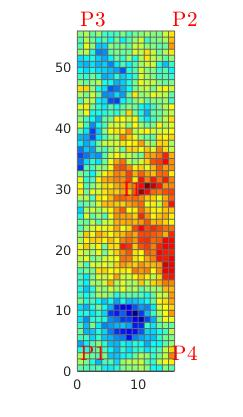
\includegraphics[width=6cm,height=6cm,keepaspectratio]
{sol1.jpg}
\caption{Solution of the SPE 10 benchmark, 16 x 56 grid cells, 2nd layer, accuracy of the snapshots $10 ^{-7}$.}
\label{fig:solspe}
\end{minipage}
\end{figure}
\newpage
\emph{SPE 10 complete}\\
We approximate the solution for the complete SPE 10 benchmark (60 x 220 x 65) with the ICCG and DICCG 
methods (see Figure \ref{fig:permspec}). The contrast in permeability between the layers for this problem is
$3 \times 10^{-7}$.
We use four deflation vectors, $z_1-z_4$ ($Configuration$ $2$).
The accuracy of the snapshots is varied from $10^{-2}$ to $10^{-11}$ in steps of $10^{-3}$. 
For the solution, accuracy is varied from $10^{-5}$ to $10^{-11}$ in steps of $10^{-3}$. Results are 
presented in Table \ref{table:spe10}. 
The convergence plot is presented in Figure \ref{fig:convspec} and the solution in Figure \ref{fig:solspec} for 
an accuracy of the snapshots and solvers of $10^{-11}$.\\
We observe from Table \ref{table:spe10}, that the number of iterations necessary to achieve convergence
is the same for ICCG and DICCG if the accuracy of the snapshots is low (tol $10^{-2}$). When the 
accuracy improves, the number of iterations is reduced for DICCG. 
Convergence is achieved within one iteration for DICCG when the accuracy of the snapshots is $10^{-11}$. 
This is a significant improvement with respect to ICCG which needs 1029 iterations to achieve the solution.\\
We also observe that, if the accuracy of the solver is not good enough, the correct solution is not reached.
This should be linked to the condition number of the matrix of the problem, and the required accuracy for the solvers. 
As the problem is very large in this case, an analysis of the condition number is not possible. However,
we know that the contrast between the permeability layers is of the order of $10^{-7}$, and from the heterogeneous
problem we can see that in this case, it is possible that the reduction of the condition number is not large enough, 
and therefore, the required accuracy is not reached. \\ 
\begin{table}[h!]
\centering
\begin{tabular}{ |p{2.5cm}|p{1.5cm}|p{1.5cm}|p{1.5cm}|} 
\hline
Tol. sol& $10^{-5}$ & $10^{-8}$ & $10^{-11}$ \\ 
\hline
  \multicolumn{4}{|c|}{Tolerance of snapshots $10^{-2}$} \\
  \hline
   ICCG        &165* &  610*& 1029\\
         DICCG  & 163*& 604* &1029 \\
    DICCG$_{POD}$& 164*& 551* &1029 \\
   \hline
     \multicolumn{4}{|c|}{Tolerance of snapshots $10^{-5}$} \\
  \hline
   ICCG&165* &  610*& 1029\\
         DICCG& 1*& 467** &878 \\
DICCG$_{POD}$& 8*& 465* &872 \\
   \hline
        \multicolumn{4}{|c|}{Tolerance of snapshots $10^{-8}$} \\
  \hline
   ICCG&165* &  550*& 1030\\
         DICCG& 1*& 1* &564 \\
         DICCG$_{POD}$& 1*& 1* &475 \\
  \hline

           \multicolumn{4}{|c|}{Tolerance of snapshots $10^{-11}$} \\
  \hline
   ICCG&165* &  572*& 1029\\
         DICCG& 1& 1 &1 \\
         DICCG$_{POD}$& 1& 1 &1 \\
  \hline

\end{tabular}
\caption{Table with the number of iterations for different accuracy in the snapshots and the solution obtained with the ICCG, DICCG and DICCG$_{POD}$ methods.}
\label{table:spe10}
\end{table}
\begin{figure}[!h]
\centering
\begin{minipage}{.5\textwidth}
 \centering
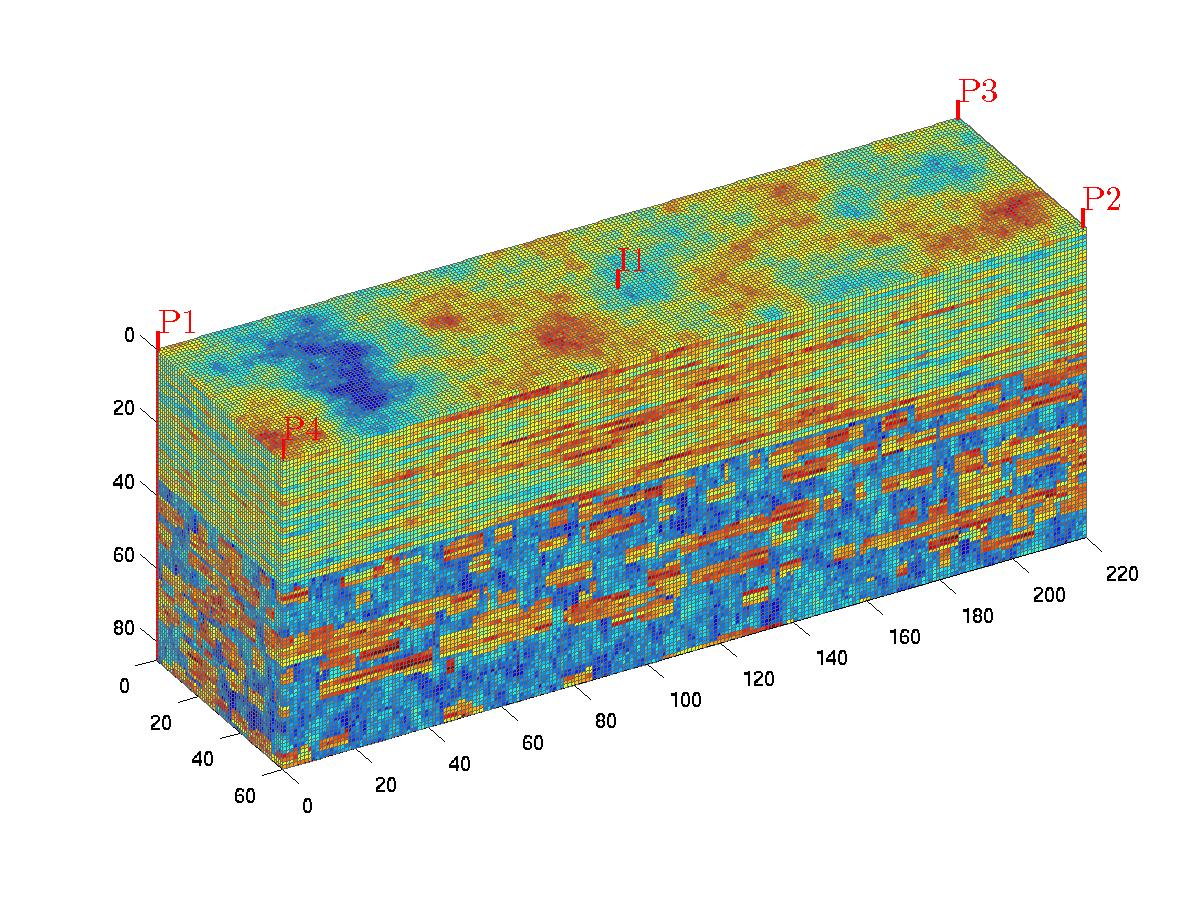
\includegraphics[width=5.5cm,height=5.5cm,keepaspectratio]
{perm_layer_.jpg}
\caption{SPE 10 benchmark, permeability field.}
\label{fig:permspec}
\end{minipage}%
\hspace{4mm}
\begin{minipage}{.45\textwidth}
 \centering
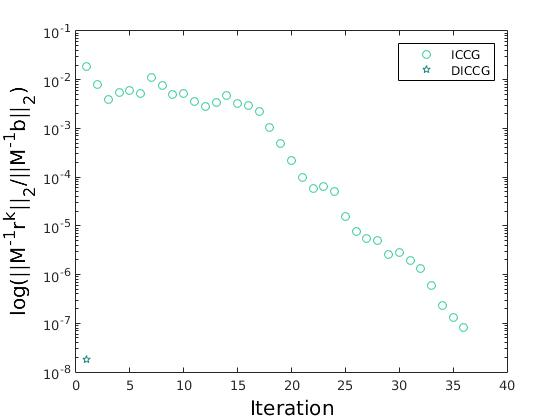
\includegraphics[width=5.5cm,height=5.5cm,keepaspectratio]
{conv_deftol-7_5_5.jpg}
\caption{Convergence for ICCG and DICCG, SPE 10 model, 85 layers, accuracy of the snapshots $10 ^{-11}$.}
\label{fig:convspec}
\end{minipage}
\end{figure}
\begin{figure}[!h]
\centering
\begin{minipage}{.6\textwidth}
 \centering
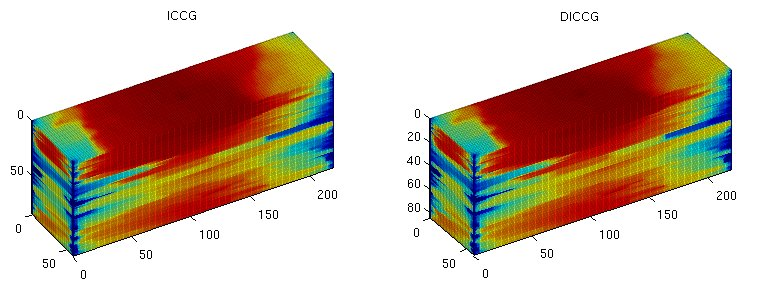
\includegraphics[width=7cm,height=7cm,keepaspectratio]
{SPE10_85_sol.jpg}
\caption{Solution to the SPE 10 model (85 layers)
with ICCG and DICCG, tolerance of the snapshots and solvers $10^{-11}$.}
\label{fig:solspec}
\end{minipage}%
\hspace{4mm}
\end{figure}
\begin{table}[!ht]
\centering
\begin{tabular}{ |p{2.5cm}|p{1.5cm}|} 

 \hline
  ICCG  & 1011\\ 
  DICCG$_{15}$  & 2000 \\ 
  DICCG$_{POD}$ & 2\\
 \hline
\end{tabular}
\caption{Table with the number of iterations for different contrast in the permeability of the layers
for the ICCG, DICCG$_{15}$ and DICCG$_{POD}$ methods, tolerance of solvers and snapshots $10^{-11}$. }
\label{table:POD15spe}
\end{table}  

For this problem, we also study the behavior of the DICCG method with 15 linearly dependent snapshots. 
The snapshots used are the same as the snapshots used for the heterogeneous 
permeability case (with 15 snapshots). The accuracy for the snapshots and the solvers is $10^{-11}$.\\
The eigenvalues of the data snapshot correlation matrix $\mathbf{R}=\mathbf{X}\mathbf{X}^T$ are presented
in Figure \ref{fig:eigspe}. The number of iterations necessary to achieve the desired tolerance 
for the ICCG and DICCG methods is presented
in Table \ref{table:POD15spe}. For the deflated method we use 15 snapshots as deflation vectors (DICCG$_{15}$), and 
the eigenvectors corresponding to the four largest eigenvalues (1-4) of the matrix $\mathbf{R}$.\\
\begin{figure}[!h]
 \centering
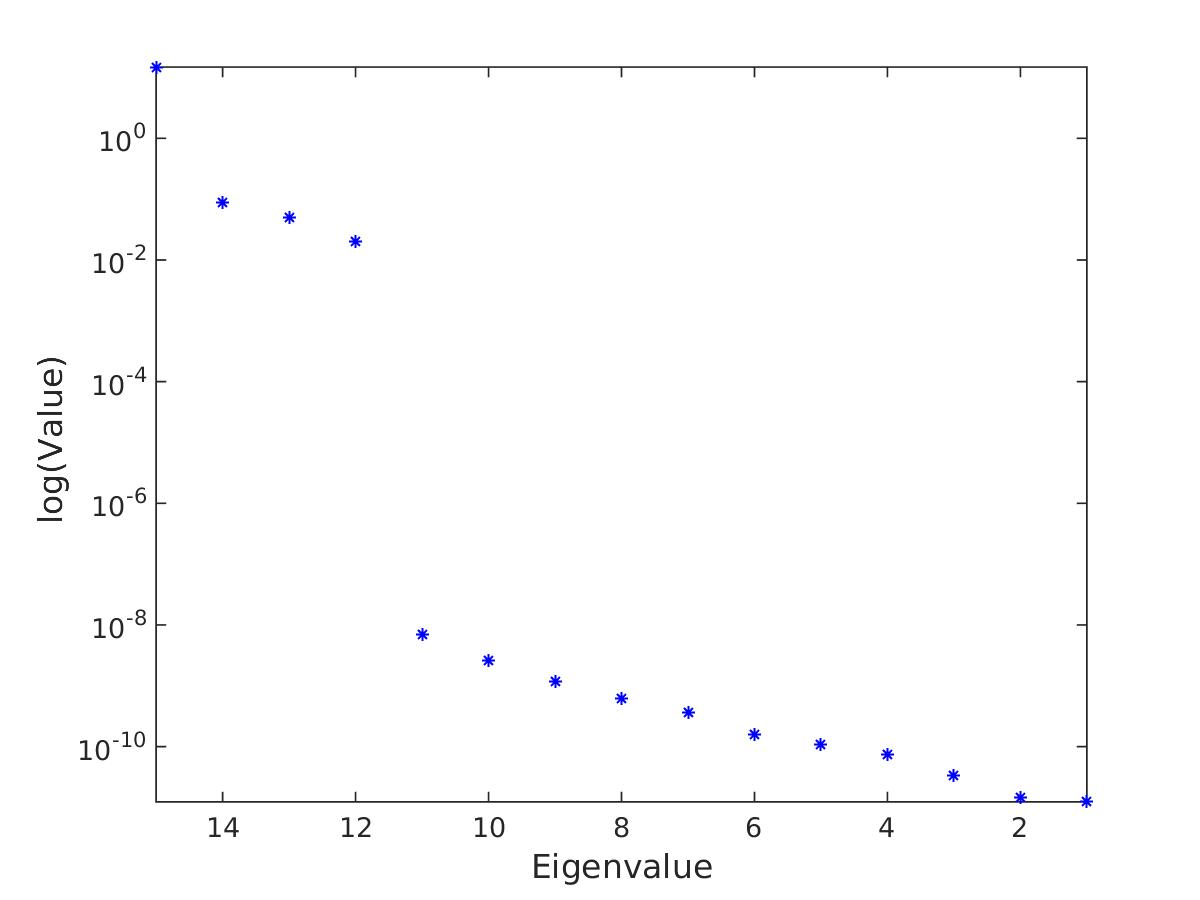
\includegraphics[width=6cm,height=6cm,keepaspectratio]
{eig_pod_spe.jpg}
\caption{Eigenvalues of the snapshot correlation matrix $\mathbf{R}=\mathbf{X}\mathbf{X}^T$, 15 snapshots used.}
\label{fig:eigspe}
\end{figure}  
We observe in Table \ref{table:POD15spe} that for the deflated method, when we use the 15 snapshots, the 
correct solution is not reached after 2000 iterations, the maximum number of iterations allowed for this problem. 
As mentioned for the layered problem with Neumann boundary conditions, this behavior is caused by the 
dependence of the snapshots. If we use 4 
of the basis vectors of POD, we reach the 
solution within two iterations. As in the heterogeneous permeability problem, we reduce the number of snapshots from 15 to 4 using 
the basis vectors of POD and we reach the solution after a small number of iterations.  
 

% \begin{figure}[!htb]
%   \centering
%   \includegraphics[width=0.6\textwidth]{....eps}
%   \caption{...}
% \end{figure}
\newpage
\newpage
\section{Conclusions}
Single-phase flow of an incompressible fluid through porous media with high-contrast in
the permeability field is studied. We study an academic layered problem and the SPE 10 benchmark.
For the solution of these problems, we propose a selection of 
physics-based deflation vectors to be used with the Deflated Conjugated Gradient 
preconditioned with Incomplete Cholesky (DICCG) method.\\Results show that the 
choice of deflation vectors is important for a good performance of the method and that the correct choice
depends on the boundary conditions. 
The proposed deflation vectors are based on snapshots, solutions of the system with some variations on the 
right-hand side. 
\\ 
Snapshots are selected taking into account the sources, wells in this case, and the boundary conditions.
When Dirichlet boundary conditions are used, vectors related to the wells and a vector related to the 
boundary conditions should be used. In the case of Neumann boundary conditions, only snapshots
related to the wells are used. Snapshots are used as deflation vectors in the case of Dirichlet and Neumann 
boundary conditions. \\
For the case with Neumann boundary conditions only, snapshots and basis vectors of POD are
used as deflation vectors. For the first set of experiments with the layered and SPE 10 problems, 
the number of snapshots depends on the number 
of wells; in these examples four snapshots are used. Results show that the performance of the DICCG method is similar when we use
four snapshots or two basis vectors of POD as deflation vectors in all the studied examples with Neumann
boundary conditions only. Although the number of snapshots is not large, in problems that require a larger 
number of snapshots to capture the dynamics of the system, POD vectors could be useful
to reduce this number. As an example, we solve the heterogeneous layered problem and the complete SPE 10 problem with a 
larger number of snapshots. We reduce the 
original set of 15 snapshots to 4 basis vectors using POD.\\
Results also show that the accuracy of the snapshots used as deflation vectors is essential for the correct 
performance of the DICCG method. 
For an academic layered problem, we note that the contrast between 
the layers modifies the condition number and demands a higher accuracy for the solvers. \\
We also observe that if the accuracy of the snapshots is not 'good' enough, the solution of the 
original system with the deflated method is reached, but the number of iterations is large, in some cases is the same as 
for the ICCG method. As the accuracy of the snapshots is improved, the number of iterations is reduced for
the deflated method.
For the cases when the correct accuracy is used for the snapshots, the DICCG method reaches the solution within 
one iteration. \\
Results also show that the performance of the solver DICCG does not depend on the grid size 
(SPE 10 example with one layer) or on the contrast between permeability layers (academic layered problem), 
when a correct accuracy for the snapshots and the solver is used.

\newpage
\appendix
\section{Appendix 1. Stopping criteria\label{a2}}
When we use an iterative method, we always want that our approximation is close enough 
to the exact solution. In other words, we require that the error \cite[pag. 42]{Saad03}: 
$$||\mathbf{e}^k||_2=||\mathbf{x}-\mathbf{x}^k||_2,$$ or the relative error: 
$$\frac{||\mathbf{x}-\mathbf{x}^k||_2}{||\mathbf{x}||_2},$$is small. \\
When we want to chose a stopping criteria, we could think that the relative error is a
good candidate, but is has the disadvantage that we need to know the exact solution to compute it.
What we have instead is the residual $$\mathbf{r}^k=\mathbf{b}-\mathbf{A}\mathbf{x}^k,$$ 
that is actually computed in each iteration of the CG method. There is a relationship between the 
error and the residual that can help us with the choice of the stopping criteria.
$$\frac{||\mathbf{x}-\mathbf{x}^k||_2}{||\mathbf{x}||_2}\leq \mathbf{C}_2(A)\frac{||\mathbf{r}^k||_2}{||\mathbf{b}||_2}.$$
With this relationship in mind, we can choose the stopping criteria as an $\epsilon$ for which
$$ \frac{||\mathbf{r}^k||_2}{||\mathbf{b}||_2}\leq \epsilon.$$
But we should keep to have in mind the condition number of the matrix $\mathbf{A}$, because the relative error will be bounded by:
$$\frac{||\mathbf{x}-\mathbf{x}^k||_2}{||\mathbf{x}||_2}\leq \mathbf{C}_2(A) \epsilon.$$
\section{Acknowledgements}

We like to thank the Mexican Insitute of Petroleum (IMP) which, through the program:  
'Programa de Captaci\'on de Talento, Reclutamiento, Evaluaci\'on y Selecci\'on de Recursos Humanos (PCTRES)',
has sponsored this work.
\bibliographystyle{unsrt}

 \begin{thebibliography}{6pt}
%   \bibitem[{<reference>}]{<cite>} ...
\bibitem{Astrid11} 
P. Astrid, G. Papaioannou, J. C. Vink and J.D. Jansen. [2011]
\textit{Pressure Preconditioning Using Proper Orthogonal Decomposition}.
Paper SPE 141922 presented at the SPE Reservoir Simulation Symposium, The Woodlands, USA, 
21-23 February.
\bibitem{Clemens04} 
M. Clemens, M. Wilke, R. Schuhmann and T. Weiland. [2004]
\textit{Subspace projection extrapolation scheme for transient field simulations}.
IEEE Transactions on Magnetics. \textbf{40}(2), 934-937.
\bibitem{Christie01}
M.A. Christie, and M.J. Blunt. [2001] Tenth SPE Comparative Solution Project: 
a Comparison of Upscaling Techniques. 
SPE Reservoir Engineering and Evaluation \textbf{4} (4): 308-317.
\bibitem{Jansen13} 
J. D. Jansen. [2013]
\textit{A systems description of flow through porous media.}
New York: Springer.
\bibitem{Mark06} 
R. Markovinovi{\'c} and J. D. Jansen. [2006]
\textit{Accelerating iterative solution methods using reduced-order models as solution predictors}.
International journal for numerical methods in engineering. \textbf{68}(5), 525-541.
\bibitem{Lie13} 
K. A. Lie. [2013]
\textit{An Introduction to Reservoir Simulation Using MATLAB:
    User guide for the Matlab Reservoir Simulation Toolbox (MRST)}.
SINTEF ICT.
\bibitem{Saad03} 
Y. Saad. [2003]
\textit{Iterative Methods for Sparse Linear Systems}.
Society for Industrial and Applied Mathematics Philadelphia. 
\bibitem{Smith96} 
B. Smith, P.  Bjorstad, W. Gropp. [1996]
\textit{Domain decomposition: parallel multilevel methods for elliptic partial differential equations}.
Cambridge University Press New York. 
\bibitem{Tang08} 
J.M. Tang. [2008]
\textit{Two-Level Preconditioned Conjugate Gradient Methods with Applications to 
       Bubbly Flow Problems}. PhD Thesis, Delft University of Technology. 
\bibitem{Tang09} 
J.M. Tang, R. Nabben, C. Vuik and Y. Erlangga. [2009]
\textit{Comparison of two-level preconditioners derived from deflation, domain decomposition and multigrid methods}.
Journal of scientific computing. \textbf{39}(3), 340-370.
\bibitem{Vuik99} 
C. Vuik, A. Segal and J. A. Meijerink. [1999]
\textit{An Efficient Preconditioned CG Method for the
                  Solution of a Class of Layered Problems with
                  Extreme Contrasts in the Coefficients}.
Journal of Computational Physics. \textbf{152}, 385-403.
\bibitem{Vuik02} 
C. Vuik, A. Segal, L.  Yaakoubi and E. Dufour. [2002]
\textit{A comparison of various deflation vectors applied 
    to elliptic problems with discontinuous coefficients}.
Applied Numerical Mathematics. \textbf{41}(1), 219. 

\end{thebibliography}
% %
% or
%


 %\bibliography{research}

\end{document} 